\documentclass[hangul, 11pt, chapter, oneside, openany]{oblivoir}

\usepackage[stock]{fapapersize}  
% 참고: http://ajt.ktug.org/2011/0501karnes.pdf
% 인용:
% 특별히 \setheadfoot, \setheaderspaces, \setmarginnotes와 같은 명령을 써야 하 는 상황이라면
% \usepackage{fapapersize}와 \usefapapersize 명령 사이에 두어야 효 과가 발생한다.
%
\usefastocksize{160mm,210mm}% 실제 인쇄되는 종이의 크기 {paperwidth}{paperheight} ipad
\setheadfoot{0mm}{3\onelineskip}% {headheight}{footskip}
\setmarginnotes{0mm}{0mm}{0mm}% {marginparsep}{marginparwidth}{marginparpush}
\usefapapersize{160mm,210mm,24mm,*,22mm,*}% 재단된 용지. 제작이 끝난 책의 크기


\usepackage{graphicx}
\graphicspath{{images/}}

\usepackage[dvipsnames, svgnames]{xcolor}
\definecolor{Beeswax}{cmyk}{0,.30,.78,0}
\definecolor{GoldenGlow}{cmyk}{.07,.31,.95,0}
\definecolor{OysterGray}{cmyk}{.16,.14,.24,0}
\definecolor{PantoneBlue}{cmyk}{.82,.29,0,0}
\definecolor{PantoneBlue2}{cmyk}{.82,.29,0,.1}
\definecolor{SunOrange}{cmyk}{0,.47,.78,0}

\makepagestyle{jeju}

% 상단 면주
\makeevenhead{jeju}{}{}{}%{left}{center}{right}
\makeoddhead{jeju}{}{}{}

% 하단 면주
% {스타일이름}{left}{center}{right}: 홀수쪽 하단 면주
\makeevenfoot{jeju}{\color{gray}\footnotesize\textsf{\leftmark}}{}{}
\makeoddfoot{jeju}{}{}{\color{gray}\footnotesize\textsf{\thepage}}

\copypagestyle{chapter}{plain}
% plain 페이지스타일을 chapter 라는 이름의 스타일로 복사.
\makeoddfoot{chapter}{}{}{\color{gray}\footnotesize\textsf\thepage}


\defaultfontfeatures{Mapping=tex-text}
\setmainfont{UnJamoBatang}%Cambria}
\setsansfont[Scale=0.8]{UnJamoNovel}
\setmonofont[Scale=0.8]{UnPen}
\setmainhangulfont[Renderer=ICU, preperiodkern=-.2pt, precommakern=-.2pt]{HCR Batang LVT}
\setsanshangulfont[Scale=1.2]{UnJamoDotum}
\setmonohangulfont[Scale=1.1]{UnJamoSora}
\newfontface\supergothic{UnTaza}
\xetexkofontregime[cjksymbols=hanja]{hangul}


\usepackage{titlesec}
\usepackage{textpos}
\titleformat{\chapter} % texdoc titlesec
	{\pagestyle{chapter}\vspace{-1cm}\normalfont\ttfamily\Huge\bfseries\color{PantoneBlue}} % PantoneBlue is custom color name.
	{}
	{0pt}
 	{\pagestyle{jeju}}

\setlength{\TPHorizModule}{1cm}
\setlength{\TPVertModule}{1cm}
\newcommand{\datebox}[1]{% texdoc textpos
	\begin{textblock}{3}(.05,-3.0)%hsize, (hpos, vpos)
		\textcolor{PantoneBlue2}{\footnotesize\sffamily{#1}}
	\end{textblock}
}

\titleformat{\section}
	{\normalfont\sffamily\bfseries\large\color{GoldenGlow}}
	{}
	{0pt}
	{}

\newcommand{\supers}[1]{%윗첨자용
	\raisebox{0.3em}{%
		\textcolor{PantoneBlue2}{\tiny{\supergothic #1}}
	}
}

\renewcommand{\thefigure}{\#\arabic{figure}}
\renewcommand{\figurename}{}
\newfixedcaption{\captionoffig}{figure}
\captionnamefont{\color{orange}\ttfamily\footnotesize}
\captiontitlefont{\color{gray}\sffamily\footnotesize}
\hangcaption
\captionstyle{\raggedright}
\precaption{\vspace{-3mm}}

\newenvironment{fillimg}[1]%
{%
	\begin{center}%
		\makebox[\textwidth]{\includegraphics[width=\paperwidth]{#1}}%
}
{\end{center}}

\setlength{\parskip}{1em}
\setlength{\parindent}{0pt}

\usepackage{titletoc}
\AtBeginDocument{\renewcommand{\contentsname}{\texttt{\HUGE{\color{gray}{11월의 역사}}}}}
\renewcommand{\cftdot}{\raisebox{.5ex}{.}}
\cftpagenumbersoff{chapter}
\setcounter{tocdepth}{1}
\setcounter{secnumdepth}{1}
\renewcommand\cftsectionleader{\color{OysterGray}\cftdotfill{\cftsectiondotsep}}
\setlength\cftchapterindent{-3.8em}
\renewcommand{\cftchapterfont}{\normalfont\ttfamily\LARGE\color{PantoneBlue}}
\renewcommand\cftsectionpresnum{}
\renewcommand\cftsectionindent{1.6em}
\renewcommand{\cftsectionfont}{\normalfont\sffamily\small\color{SunOrange}}
\renewcommand{\cftsectionpagefont}{\sffamily}
\titlecontents{section}
[1.6em]
{\sffamily\sffamily\small}
{\color{Beeswax}}
{\hspace*{0.8em}}
{\color{OysterGray}\titlerule*[1pc]{.}\color{gray}\ttfamily\contentspage}

% 차례에서 장 번호 없애기
\def\hchaptertitlehead{}

%toc 면주에 쪽번호가 달리지 않도록.
\AtBeginDocument{\addtocontents{toc}{\protect\thispagestyle{empty}}} 

\usepackage{hyperref}
\hypersetup{
    pdftitle={My LaTeX Template},
    pdfsubject={재사용을 위한 레이텍 템플릿},
    pdfauthor={b1tk3y},
    pdfkeywords={키워드, b1tk3y, XeLaTeX, Oblivoir, KTUG}
}


\title{\LaTeX, 나만을 위한 \LaTeX~ 템플릿}
\author{b1tk3y}
\date{\today}

\begin{document}

\maketitle

\begin{abstract}
문서를 구성하는 각 요소를 모듈처럼 분리하여
나중에 바꾸고 싶은 부분만 바꿔서 활용할 수 있게 만든 \LaTeX~문서작성 샘플 코드.
본문과 그림은 위키백과에서 가져왔다.
\end{abstract}

\clearpage

\tableofcontents*

\pagestyle{jeju}
\chapter{프랑스혁명}
\datebox{1789년 5월 5일}
\section{삼부회 소집}
루이 16세는 시민들의 불만을 잠재우려 재정 개혁을 단행하려 하였다. 재무 장관이었던 샤를 알렉상드르 드 칼론은 명사회를 소집해 특권 계층에게도 세금을 부과하는 개혁안을 제시하였다. 그러나 자신들의 기득권을 침해받을 것을 우려한 귀족들은 개혁안을 거부하고, 삼부회를 소집할 것을 요구하였다. 1789년의 삼부회가 열리던 당시의 상황은 심각하였다. 1788년의 흉작과 혹독한 겨울로 인한 고통이 전국토를 휘감았다. 정부는 나약했으며 멸시받고 있었다. 관리들은 불복종이 표출되는 것을 진압하기를 두려워하거나 망설이고 있었다. 대의원들에게 주어진 서면 지시 사항은 정치적 · 사회적 · 경제적 관심들을 총망라한 것이었으며 아주 많은 변화를 요구하고 있었다. 이러한 소란 가운데, 왕과 그의 신하들은 여전히 수동적인 자세였다. 그들은 삼부회가 개별적으로 열려야 할지 아니면 함께 종합적으로 고민해야 할지 하는 문제도 결정하지 못했다. 1789년 5월 5일 루이 16세는 베르사유 궁전의 살 데 메뉘 플레지르(Salle des Menus Plaisirs)에서 삼부회를 소집하였고, 귀족 188명, 성직자 247명, 평민 500명이 대의원으로 선출되었다. 재무총감 네케르는 재정의 조건을 전제로, 몇 가지 작은 개혁안을 제안하였다. 그러나 표결방식을 둘러싸고 귀족, 성직자 대표와 평민 대표 간에 갈등이 생겼다. 국새상서(國璽尙書)인 샤를 루이 프랑소와 드 폴 드 바렝탕Charles Louis François de Paule de Barentin)은 그들이 신분별로 또는 인원수대로 투표할 수 있는 것을 선택할 수 있다고 알려왔다. 제삼부회(Tiers État)는 회의를 개별적으로 할지 모여서 할지도 결정하지 못한 것에 대해서 실망하였다. 귀족들 중 일부와 하위직 성직자들의 다수는 실질적인 개혁이 필요하다고 주장하는 제삼부회에 동의하였다고 알려졌다. 합동 회의를 개최한다면, 다수를 차지하는 평민 계급은 개혁, 특권의 폐지와 부동산에 대한 중세적 권리의 폐지를 통과시킬 것이었다. 분리 회의를 하는 경우, 귀족의 대부분과 상급 성직자는 개혁을 제한하려고 할 것이었다. 따라서, 삼부회를 합동으로 개최하자는 것이 제삼부회의 첫 번째 의제로 부각하였다. 귀족, 성직자 대표는 신분별 표결 방식을, 평민 대표는 머리수 표결 방식을 지지함으로써 자신들이 속한 계급에 유리한 방향으로 회의를 이끄려고 한 것이다.

\section{바스티유 감옥 습격}
왕당파가 제헌국민의회의 무력 탄압을 기도하여, 지방으로부터 군대를 결집하고 있다는 것이 전해지자, 1789년 7월 12일부터 군대와의 사이에 충돌을 반복하였다. 7월 14일 아침, 파리 민중들은 혁명에 필요한 무기를 탈취하기 위하여 바스티유 감옥을 습격하였다. 민중들은 도개교(跳開橋)를 내리고 감옥으로 쇄도하여, 감옥을 점령하였다. 이 습격의 성공은 바야흐로 혁명의 도화선이 되었다. 이들이 프랑스 대혁명에 가담한 이유는 기득권층들에 대한 감정적인 불만이나 부르주아의 선동 때문이 아니라, ``자연으로 돌아가자''면서 평등사회를 추구한 장 자크 루소의 영향으로 불평등한 사회체제에 저항하는 사회개혁의지를 갖고 있었기 때문이다.실제로 유럽에서는 시민혁명의 영향으로 민중이 지배계급에 저항하는 권리인 저항권을 헌법으로 존중한다. 덕분에 혁명의 불길은 지방까지 확산되었다. 8월 4일에 제헌국민의회는 봉건적 특권이 폐지되었음을 선언하고, 1789년 8월 26일에는 프랑스 인권 선언을 채택하였다.

\begin{figure}
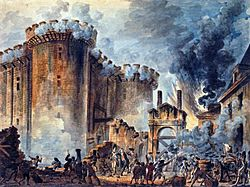
\includegraphics[width=\textwidth]{Prise-de-la-Bastille}
\captionoffig{시민들에게 공격받는 바스티유 감옥}
\end{figure}

그러나 국왕이 제헌국민의회의 선언을 인정하지 않았다. 정치적인 혼란과 전년 흉작의 영향으로 파리의 물가가 상승하기 시작하자 1789년 10월 5일 파리의 수많은 여성들이 무기를 들고 빗속에서 파리 시청 앞 광장에 모여 베르사유 궁전에 난입하여 국왕과 의회에 음식을 요구하는 생존권 투쟁을 하였다. 이들의 압력으로 루이 16세는 압력을 받아 프랑스 인권 선언을 인정하고 그녀들에게 이끌려 파리 튈르리 궁전에 가족과 함께 이주당한다. 이후, 루이 16세 일가는 파리 시민의 감시 속에서 살게 된다.

이 시기의 혁명은 온건한 미라보, 라파예트 등 입헌군주제를 지지하는 온건파 혁명주의자들에 의해 주도되고 있었다. 시민군은 자유주의 귀족 라파예트를 총사령관에 임명하고, 1790년, 그의 제안에 따라 삼색기\supers{현재 프랑스 국기}가 혁명의 깃발이 되었다.

\section{바렌느 사건}
혁명 발발로 귀족과 성직자 등 특권 계급의 대부분이 국외로 망명하기 시작하였다. 1791년 국왕과 민중의 중개자인 미라보가 죽자, 과격한 혁명을 거부한 루이 16세는 마리 앙투아네트의 친한 관계에 있는 스웨덴 귀족 페르센의 도움을 받아, 왕비의 친정인 오스트리아로 피신할 계획을 세웠다.

1791년 6월 20일, 파리를 탈출한 루이 16세 일가는 국경 앞의 바렌느에서 민중들에게 발각되어, 6월 25일 파리로 되돌아왔다. 이 사건은 프랑스 국민들에게 충격을 주었고, 동시에 루이 16세의 반혁명 의도가 폭로되었다. 혁명의 파급을 두려워하는 오스트리아와 프로이센은 8월 27일 《필니츠 선언》을 발표하여, 루이 16세의 지위를 보장하지 않으면 전쟁을 하겠다고 위협했기 때문에 루이 16세는 국왕에 머물게 되었다. 하지만 그때까지는 비교적 많은 수를 차지하고 있던 국왕 옹호파 민중의 지지를 상실하였다.

\begin{fillimg}
{Duplessi-Bertaux-Arrivee-de-Louis-Seize-a-Paris}
\end{fillimg}

프랑스 혁명은 일시적인 충격을 넘어,결코 소멸될 수 없는 확고한 성과를 남겼다. 여러 `혁명문서'가 그것을 선언적으로 제시했다. 1789년 8월 26일 `인권선언', 1791년의 헌법, 1793년의 헌법, 1795년의 헌법이 바로 그것이다. 1791년의 헌법이 입헌군주제를, 1793년의 헌법과 1795년의 헌법이 공화주의를 선언했는가 하면, 보통선거제를 규정한 1793년의 헌법과 1791년과 1795년의 헌법은 진일보한 민주주의의 가치를 드러냈다. `인권선언'과 세 헌법은 자유,평등,박애라는 자연권의 보편적 적용을 통해 새로운 사회 및 세계가 나아가야 할 실질적이고 위대한 원리를 천명했다.


\chapter{광주 학생 항일 운동}
\datebox{1929년 11월 3일}
\section{사건의 배경}
일제는 조선인들을 우민화하기 위해 고등교육 제한, 직업교육과 일본어·일본사 교육 등을 실시하였고, 학생들의 자유로운 토론과 비판, 자치활동 금지, 조선인 학생에 대한 무시, 교육자답지 못한 행동으로 조선 학생들을 억압하였다.

결국 조선인 학생들은 일본인 교육자들의 억압과 무시 그리고 우민화정책을 당하면서 항일의식을 갖게 되었다. 광주소재 각 고등보통학교(중고통합과정)에는 성진회, 독서회 등의 비밀학생조직이 생성되어 있었다. 또한 일본인 학생들에 의한 조선인 학생들의 차별, 무시 역시 학생들의 분노를 촉발하는 원인이 됐다.

1926년 4월 순종의 사망으로 6.10만세운동이 전개된다. 1926년 연말이 다가오자 민족운동과 사회주의운동내에서는 일본에 의한 자치주의에 현혹되지 말고, 흩어진 민족의 역량을 통합할 필요성이 제기된다. 이러한 흐름은 홍명희, 송진우 등의 여러 지도자들에게도 반영되었고 민흥회 등에 반영된다. 사회주의그룹에서도 정우회선언 등을 통해 분열적 종파주의로부터 좌우합작으로 나아갈 것이 결의된다. 그 결과 1927년 2월 조선일보 사장 이상재를 회장으로 동아일보의 송진우를 비롯해 허헌, 김병로, 한용운 등 국내에서 활동하고 있던 좌익-우익의 지도자들의 합작에 의해 민족단일당인 '신간회'가 조직된다. 광주학생독립운동이 터지게 되는 1929년의 연초에는 신간회의 지회가 144개, 회원은 3만9천여 명에 달해 각 지역의 청년, 노동, 농민운동을 지도해 갔다.

광주 지역에서도 1927년 10월 신간회 광주지회가 설립되었으며, 1927년 11월 전남청년연맹에서 광주청년동맹이 분리되어 결성되었다. 신간회 광주지회와 광주청년동맹의 주요 임원들은 성진회, 독서회 등의 비밀학생조직의 배후 인물이었다.

\section{광주 학생 운동의 진행}
식민지 어느 지역에서도 한일간의 감정은 존재했다. 도심의 중심지의 노른자위 땅을 차지하고 정치와 경제적 특혜를 누리며 조선인에 대한 차별과 멸시를 일삼는 식민지의 삶은 고스란히 학생들의 생활 속에도 그대로 나타났다. 넓은 평야가 있는 나주의 경우에도 경제적 부를 독점하는 것은 일본인 대지주들이었고, 그들의 자녀들은 부유를 누리며 광주로 통학하고 있었다. 가난한 조선인 학생들은 차별과 멸시 속에서 항일 의식을 키우며 광주로 통학하고 있었다.

1929년 10월 30일 나주역에 도착한 광주발 통학열차에서 내린 일본인 중학생들은 광주여자고등보통학교 학생인 박기옥·암성금자·이광춘의 댕기머리를 잡아당기며 희롱하였다. 이 광경을 목격한 박기옥의 사촌동생 박준채는 분노하여 항의했으나 말을 듣지 않자 난투극이 벌어졌다. 이 난투극은 일본인 학생 50명과 한국인 학생 30명이 싸웠는데 한국인 학생 30명이 사기면에서는 더 유리하였다.

이를 본 일본 경찰들이 일본인 학생 편을 들고, 광주고보 학생들은 차별에 대해 집단항의하였다. 이에 일본인 기업인들이 동인도회사를 모방한 식민지 수탈기관인 동양척식주식회사를 설립하고 수탈하는 것에 대해 쌓여오던 분노가 겹쳐서 폭발하게 된다. 이를 접한 1929년 11월 3일 허정숙은 광주로 내려와 이들 학생들을 면담하고 경성 지역의 여학생들 여성 운동가들을 찾아다니며 시위를 할 것을 촉구하였다.

\section{제1차 광주학생운동}
1929년 11월 3일(일요일)은 일본에게는 메이지유신의 상징인 메이지 천황의 탄생을 축하하는 명치절(明治節)이었지만, 조선인들에게는 음력 10월 3일 즉, 단군의 고조선 건국을 기념하는 개천절이었다. 한국인의 시조를 기념하는 날에 일본 천황의 생일을 일본 국가인 '기미가요'를 불러서 축하해야 하는 상황이 벌어지자 조선인 학생들은 침묵으로 일관했다. 그리고 하교길에 일본인 학생들과의 충돌사건을 불공정하게 보도한 광주일보에 몰려들어가서 항의할 정도로 그들의 반일감정은 폭발하기 시작했다.

그런데 광주고등보통학교의 조선인 학생이 광주중학교의 일본인 학생들에게 테러당하는 일이 벌어지면서 폭력사태까지 발생하였다. 한편 장재성 등은 일제에 대항할 자세한 행동방향을 제시한다.

\begin{enumerate}
\item 우리의 투쟁 대상은 광주중학생이 아니라 일본 제국주의이니 투쟁 방향을 일제로 돌릴 것.
\item 광주중학생에 대한 적개심과 투쟁을 일제에 대한 증오와 독립투쟁으로 바꿀 것.
\item 광주중학생과 대치 중인 광주고보생을 해산시키지 말고 광주고보로 집합시켜 적개심에 불타는 학생들을 식민지 강압정책 반대 시위운동으로 돌릴 것.
\item 장재성이 시위운동을 직접 지도할 것.
\item 우리는 앞으로 다른 동지들과 연락하여 다음 투쟁을 준비하고 계획할 것.
\end{enumerate}

그리하여 장재성의 주도로 학생들은 광주농고 학생들과 함께 광주시민들의 지지를 받으며 용감히 적(일제)을 물리치자는 내용의 행진가를 부르는 가두시위를 하였다. 일제는 항일시위에 가담한 70여 명의 조선인 학생 중 60여 명을 구속, 검사국으로 송치하는 탄압을 하였고 심지어는 개인의원인 태양의원에서 치료받던 학생들을 도립병원장이 치료할 가치도 없다면서 비하하는 망언을 하여 공분을 샀다. 동아일보, 조선일보 등에서도 일제의 학생운동 탄압과 차별을 비판하는 기사를 보도할 정도였다.

\begin{figure}
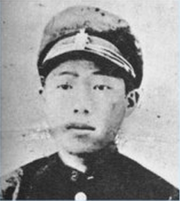
\includegraphics[width=0.65\textwidth]{gwangju3}
\captionoffig{당시 열차에서 일본인 학생들과 싸우던 박준채}
\end{figure}

장재성은 광주학생들을 설득하는 유인물을 작성했으며, 인쇄를 맡은 오쾌일에 의해서 등사판을 이용하여 박기석의 집에서 약 1,000장을 인쇄하였다. 그리고 1929년 11월 12일 오전 8시 경 오쾌일은 광주고보와 광주농고의 학생들을 통해서 유인물을 배포한다. 당시 광주여자고등보통학교의 여학생들도 교정에서 시위에 가담하였으며, 광주고보, 광주농고, 광주여자고보 학생들은 동맹휴학으로 일제에 대항하였다. 일제는 250여 명에 가까운 학생들을 검거했으며, 사회운동단체 간부들도 검거당했다. 일단 경찰에 구속된 학생들에 대해서는 학교당국의 가혹한 처벌이 잇따랐다. 거의 대부분의 학생들이 무기정학, 퇴학으로 광주학생운동 가담자들을 탄압함으로써 중등학교 학교 교실이 텅빌 지경이었다. 일제는 12월 28일까지 언론통제를 단행하여 학생운동의 확산을 차단하고, 전국적 항일운동으로 확대발전하는 것을 막으려고 했지만,오히려 각종 탄압에 대한 소문과 풍문이 더욱 커지면서 그동안 웅축되었던 항일활동이 폭발적으로 증가하는 계기를 제공했을 뿐이다. 당시 학생운동의 전개과정은 "약소민족해방만세!, "제국주의타도 만세!, 피압박 민족 해방 만세!, 무산계급혁명 만세!"라는 구호를 사용하여 일제 경찰이 사상운동으로 몰아붙일 만큼 학생운동의 지도부들은 당시 러시아혁명 이후 유행하던 사회주의 이론에 적잖은 영향을 받았다. 학생운동의 원동력은 무엇보다 민족적 차별과 억압에 맞서야 한다는 자연스러운 분노와 우리 민족의 독립적 삶을 되돌려야 한다는 의기에 바탕을 둔 건강한 청년정신으로부터 발로했다고 볼 수있다

\section{학생독립운동의 전국 확산}
신간회 광주지회의 상무간사였던 장석천은 11월 16일 서울로 올라와 조병옥, 김병로 등 신간회 중앙간부들에게 제2차 시위의 전말을 보고하고, 이어 조선청년동맹 중앙간부 곽양훈, 차재정 등에게 광주학생들의 항일시위를 전국 항일 시위 운동으로 확산할 것을 역설했다. 이 두 모임에서 서울 시내 각 학교에 이미 조직되어 있는 비밀독서회 조직을 통해 시위운동을 서울로 확산하기로 결정하였다. 장석천은 특별히 휘문고보 5년생이었던 후배 장홍염을 설득하여 장홍염이 서울시내의 주요 조선인학교들의 학생운동가들을 접촉하였다. 장홍염 자신이 1년 전에 'ㄱ당 사건'에 관련되어 수개월간의 옥고를 치르고 석방된 처지였다. 11월 20일부터 12월 2일까지의 준비기간을 거쳐 1929년 12월 3일 서울의 각 학교의 조선인 학생들에게는 광주학생들의 시위운동에 대한 전말과 독립운동에의 동참을 호소하는 격문이 모두 뿌려졌다.

\begin{figure}
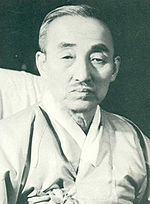
\includegraphics[width=.705\textwidth]{Kimbyungro}
\captionoffig{광주 학생 운동 관련자들을 변호한 김병로 변호사}
\end{figure}

일본 경찰의 예비검속으로 서울 지역의 조직 주동자들이 잡혀 갔지만, 드디어 12월 9일부터 서울지역 학교들의 항일시위가 시작되었다. 12월 9일에는 경신학교 학생 300여 명, 보성고보 학생 400여 명, 중앙고등보통학교 700여 명, 휘문고등보통학교 학생 400여 명, 협성실업학교 학생 150여 명이 시위에 참가하였다. 12월 9일 하루에만 1,200여 명의 시위학생들이 경찰에 체포되었다. 이후 12월 13일까지 서울지역에서만 1만 2000여 명의 학생이 시위, 동맹휴학에 참여하였고, 그중 1,400여 명이 체포되었다. 그중 서울 지역에서만 45명이 구속되고, 이 가운데 35명이 최종적으로 재판에 회부되었다.

당시 신간회는 이 광주학생 시위운동을 전국적 항일독립운동으로 확산시키기 위해 12월 10일 권동진(3.1운동시 33인중 1인), 허헌, 동아일보사장 송진우, 조선일보 부사장 안재홍, 조병옥, 홍명희, 한용운, 주요한 등이 대책회의를 갖고, 12월 13일 광주학생사건 진상발표회를 갖고, 곧바로 군중을 선동하여 시위 운동을 갖고, 지방지회에도 동일한 행동을 하도록 지시한다는 방침을 결정했다.

일본경찰이 이를 탐지하고 12월 13일 아침 6시 신간회 주요간부 30여 명을 예비검속하여 서울의 진상발표회는 열리지 못했지만, 지방지회에 보내는 지시문은 이미 전달되어 이후 전국 각 지역에서 1930년 3월초까지 학생들을 중심으로 항일시위 만세운동이 계속되었다. 이 학생독립운동은 만주지역의 한인 거주지역까지 확대되었다. 참가학교 총수에 대한 일제총독부의 기록은 처음에는 194개로 나타났으나 이후 참여학교에 대한 조사를 통해 광주광역시교육청에서는 2006년에 총 320개의 학교를 찾아내었으며, 이후 학생독립운동기초자료발굴팀등에 의해 350여개의 조선인관련 학교가 참여하였고 일본과, 중국, 러시아, 미국 등의 해외학교나 해외단체를 포함할 경우 참여규모에 대해서는 좀더 확대해 설명할 수 있다는 주장도 제기되고 있다.

또한 참여인원의 경우에도 학생이 주축이기는 하지만, 각종청년단체, 노동단체, 신간회, 해외 독립운동단체, 해외 피압박민족해방운동관련 옹호 지지운동단체, 반제동맹이나 중국공산당, 중국국민당의 각종 기관들, 해외조선인들이 만든 재만한족연합회와 같은 기성단체를 포함하면 규모나 역할, 국제적 성격은 1929년 세계정치의 역사 속에서 매우 중요한 의미를 가진다고 할 수있다.


\end{document}
